\documentclass{article}
\usepackage[UTF8]{ctex}
\usepackage{float}
\usepackage{graphicx}

\title{Bellman-Ford 算法的实现}
\author{林敬翊}
\date{2022年12月14日}

\begin{document}

\maketitle

\section{设计思路}
在graph中添加BellmanFord的算法 \\
~\\
在这函数中,需要提供顶点和边数和权重。
~\\
以下为图
\begin{figure}[htb]
    \centering
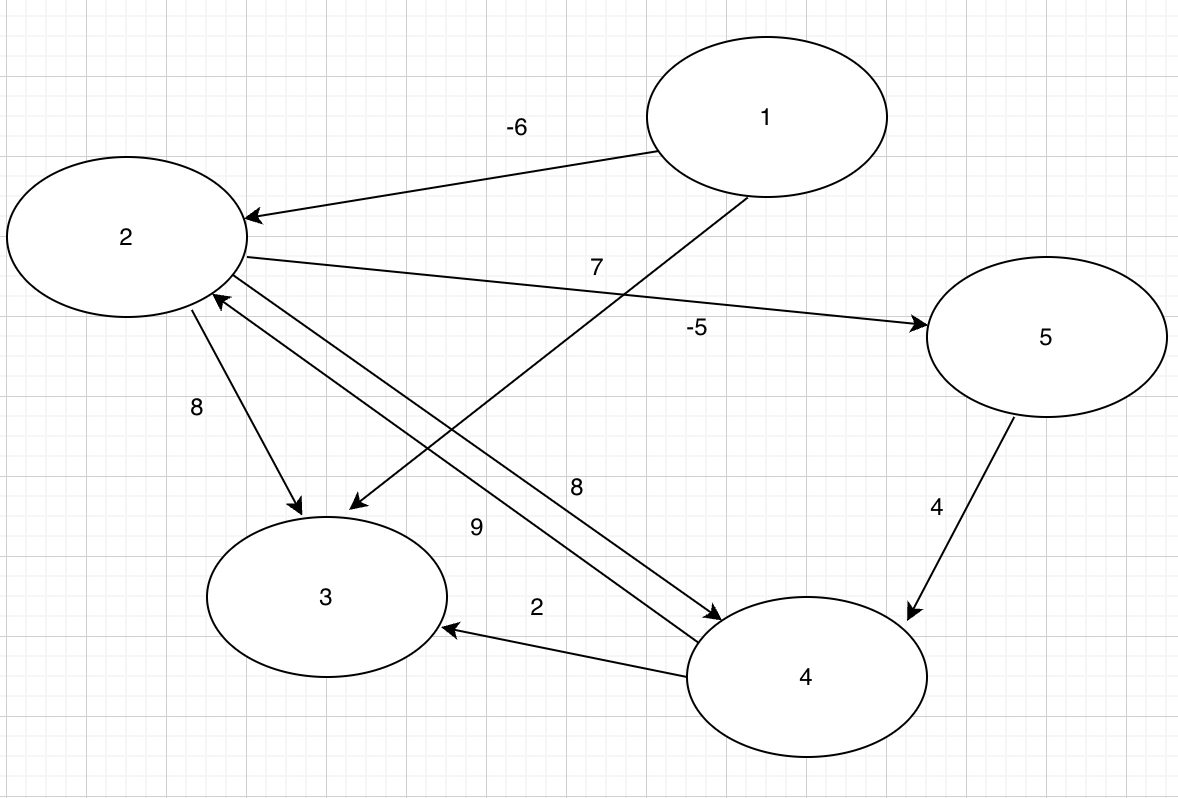
\includegraphics[width=10cm]{graph.png}
    \end{figure}
    
\section{测试结果}
当产生负边环,将跳出“Graph contains negative weight cycle”。

会出现2147483647的原因是因为属于infinity,无法抵达该点





\begin{figure}[htb]
    \centering
\begin{minipage}[t]{0.48\textwidth}
    \centering
    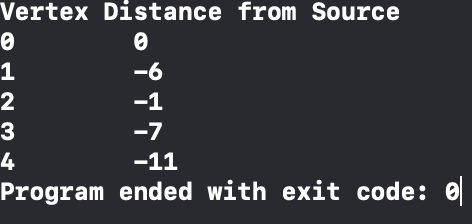
\includegraphics[width=5cm]{1.png}
    \caption{以1为起点}
\end{minipage}
\begin{minipage}[t]{0.48\textwidth}
    \centering
    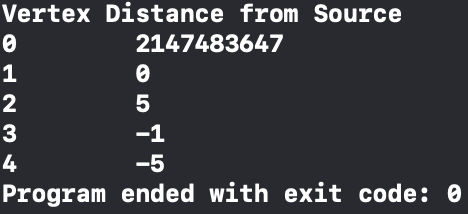
\includegraphics[width=5cm]{2.png}
    \caption{以2为起点}
\end{minipage}
\end{figure}

\begin{figure}[htb]
    \centering
\begin{minipage}[t]{0.48\textwidth}
    \centering
    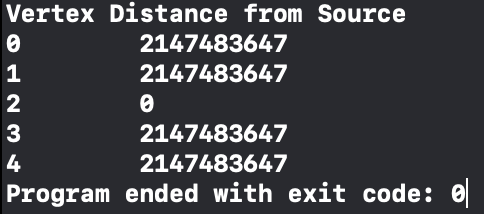
\includegraphics[width=5cm]{3.png}
    \caption{以3为起点}
\end{minipage}
\begin{minipage}[t]{0.48\textwidth}
    \centering
    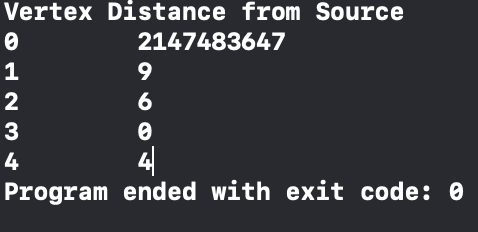
\includegraphics[width=5cm]{4.png}
    \caption{以4为起点}
\end{minipage}
\end{figure}



\end{document}
